%% linop.sty
%% Copyright 2016 Johannes Weytjens
%
% This work may be distributed and/or modified under the
% conditions of the LaTeX Project Public License, either version 1.3
% of this license or (at your option) any later version.
% The latest version of this license is in
%   http://www.latex-project.org/lppl.txt
% and version 1.3 or later is part of all distributions of LaTeX
% version 2005/12/01 or later.
%
% This work has the LPPL maintenance status `maintained'.
% 
% The Current Maintainer of this work is Johannes Weytjens
%
% This work consists of the file linop.sty

\documentclass[10pt]{article}

% layout
\usepackage[T1]{fontenc}
\usepackage[utf8]{inputenc}
\usepackage[a4paper]{geometry}
\usepackage[english]{babel}
\usepackage[tracking=true,kerning=true,factor=1250]{microtype}
\usepackage[compact]{titlesec}
\usepackage{tocloft}
\usepackage[charter,expert]{mathdesign}
\usepackage[scaled=0.96]{XCharter}
\usepackage{linop}
\usepackage{parskip}
\usepackage{float}
\usepackage{xparse}
\usepackage{fancyvrb}
\usepackage{booktabs}
\usepackage{graphicx}
\usepackage{caption}
\usepackage{cprotect}
\usepackage[hang]{footmisc}

% math
\usepackage{bm}

% titlesec
\titleformat{\section}[hang]{\scshape\Large}{\thesection.}{1ex}{}
\titleformat{\subsection}[hang]{\scshape\large}{\thesubsection.}{0.5ex}{}
\titleformat{\subsubsection}[hang]{\scshape}{\thesubsubsection.}{0.25ex}{}

% tableofcontents
\setcounter{tocdepth}{1}
\renewcommand{\cfttoctitlefont}{\Large\scshape}
\renewcommand{\cftsecfont}{\scshape}
\renewcommand{\cftsecpagefont}{\large}

% footmisc
\setlength{\footnotemargin}{1em}

% distance between columns in a table
\setlength{\tabcolsep}{20pt}

% caption
\DeclareCaptionFormat{center}{{\centerline{#1#2}\\}#3}
\captionsetup{font={small},labelfont=sc,width=0.8\textwidth,format=center,labelsep=none,justification=justified}

% microtype
\SetTracking{encoding={*}, shape=sc}{0} % small caps are correctly typeset
% protrusion for footnotes
\DeclareMicrotypeSet{textandfootnote}{%
  encoding = {OT1,T1},
  family = {*},
  size = {normalsize,footnotesize,small,large,Large,scriptsize},
  font = {*}
}

% PDF (metadata)
\usepackage{hyperref}
\hypersetup{
    pdfauthor = {Johannes Weytjens},
    pdftitle = {The linop package v0.1},
    pdfcreator = {LaTeX}
}

\title{The \texttt{linop} package v0.1}
\author{Johannes Weytjens \\ \href{johannes.weytjens@nietsissimpel.org}{johannes.weytjens@nietsissimpel.org}}

\begin{document}
\maketitle

\tableofcontents

\section{Introduction}
There exist already many packages to help you typeset common and less common mathematical notation with ease. Yet, to the best of my knowledge, there does not yet exist a package that provides an easy way to typeset operators as they appear for example in many body physics, quantum (field) theory or linear algebra. The aim of this package is to provide two simple commands and many options to easily write operators in any of the ways they commonly appear.

Besides providing easy to use macros, this package also ensures consistent spacing for subscript and superscript. To illustrate this point, compare the normal way for typesetting operators with the macros provided by this package.

\begin{table}[ht]
	\centering
	\begin{tabular}{ll}
		\verb|\hat{a}_{in}\hat{a}_{in}^{\dagger}| & $\hat{a}_{in}\hat{a}_{in}^{\dagger}$ \\
		\verb|\op{a}{in}\hc{a}{in}| & $\op{a}{in}\hc{a}{in}$
	\end{tabular}
\end{table}

Typesetting the \verb|\dagger| and a subscript simultaneously pushes the subscript down, this is no longer the case with the here defined macros.

\subsection{Required packages}
As these are simple macros, you only need the \texttt{xparse} package.

\newpage
\section{List of commands}
The two macros defined in this package are \verb|\op| and \verb|\hc| as well as their starred versions.

\begin{Verbatim}[commandchars=\&\"\!]
	\op[&rmfamily&itshape"superscript spacing!&ttfamily]{&rmfamily&itshape"operator!&ttfamily}{&rmfamily&itshape"subscript!&ttfamily}{&rmfamily&itshape"superscript!&ttfamily}{&rmfamily&itshape"supersuperscript!&ttfamily}
	\hc[&rmfamily&itshape"superscript spacing!&ttfamily]{&rmfamily&itshape"operator!&ttfamily}{&rmfamily&itshape"subscript!&ttfamily}{&rmfamily&itshape"superscript!&ttfamily}{&rmfamily&itshape"supersuperscript!&ttfamily}
\end{Verbatim}

These macros typeset an operator and the Hermitian conjugate respectively. Only the \emph{operator} argument is mandatory, all other arguments can either be empty or be skipped entirely if no subscript or superscript is desired. The optional argument \emph{superscript spacing} only applies to the starred versions. Supersuperscripts are implemented to distinguish between e.g.\ the order in some expansion and the square of the operator.

\begin{table}[H]
	\centering
	\begin{tabular}{ll}
		\verb|\op{a}{in}{0}| & $\op{a}{in}{0}$ \\
		\verb|\op{a}{}{(1)}{2}| & $\op{a}{}{(1)}{2}$ \\
		\verb|\hc{b}{out}{0}| & $\hc{b}{out}{0}$ \\
		\verb|\hc{b}{out}{}{2}| & $\hc{b}{out}{}{2}$ 
	\end{tabular}
\end{table}

The defaults style is to typeset all operators with a hat. The none starred versions use \verb|\hat| and are only appropriate for single symbol operators. The starred version use \verb|\widehat| which scales with the width of the operator and can therefore be used for wider symbols. The \verb|\widehat| often overlaps with the superscripts however, so the starred version insert a \verb|\>| before the superscripts and a \verb|\:| for the Hermitian conjugate superscript. Controling the spacing of the superscript for individual operators can be done with the optional \emph{superscript spacing} argument.

\begin{table}[H]
	\centering
	\begin{tabular}{ll}
		\verb|\op*{A}{in}{0}| & $\op*{A}{in}{0}$ \\
		\verb|\hc*{ab}{out}| & $\hc*{ab}{out}$ \\
		\verb|\hc*[\kern4pt]{\mathcal{L}}| & $\hc*[\kern4pt]{\mathcal{L}}$ 
	\end{tabular}
\end{table}


\section{List of options}
\subsection{bold}
Some prefer to use bold letters for operators instead of hats. This can be achieved by using the \texttt{bold} option when loading the package. When using this option, the starred versions will produce the same result as the none starred versions.

\renewcommand{\linopstyle}{\mathbf}
\renewcommand{\linopstylewide}{\linopstyle}

\begin{table}[H]
	\centering
	\begin{tabular}{ll}
		\verb|\op{a}{in}{0}| & $\op{a}{in}{0}$ \\
		\verb|\hc{b}{out}| & $\hc{b}{out}$
	\end{tabular}
\end{table}

\subsection{bmbold}
The \texttt{bmbold} option achieves the same effect as bold, but instead uses the bold math font provided by the \texttt{bm} package.

\renewcommand{\linopstyle}{\bm}

\begin{table}[H]
	\centering
	\begin{tabular}{ll}
		\verb|\op{a}{in}{0}| & $\op{a}{in}{0}$ \\
		\verb|\hc{b}{out}| & $\hc{b}{out}$
	\end{tabular}
\end{table}

\subsection{nohat}
The option \texttt{nohat} typesets the operators without a \verb|\hat|. This also applies to the starred versions.

\renewcommand{\linopstyle}{}

\begin{table}[H]
	\centering
	\begin{tabular}{ll}
		\verb|\op{a}{in}{0}| & $\op{a}{in}{0}$ \\
		\verb|\hc{b}{out}| & $\hc{b}{out}$ 
	\end{tabular}
\end{table}

\subsection{wide}

\renewcommand{\linopstyle}{\hat}
With the wide option, all operators will use \verb|\widehat|, regardless of whether you're using the starred or non starred versions.

\subsection{star}

\renewcommand{\linopconjugate}{*}

The \texttt{star} options typesets the Hermitian conjugate with a star instead of a dagger.

\begin{table}[H]
	\centering
	\begin{tabular}{ll}
		\verb|\hc{b}{out}| & $\hc{b}{out}$
	\end{tabular}
\end{table}



\subsection{compact}
The consistent spacing is provided by using \verb|\mathstrut| in both the subscript and superscript. As the misalignment is caused by using a \verb|\dagger| in the superscript, the same effect can be achieved by using a \verb|\phantom{\dagger}| in the superscript of the non Hermitian conjugated operator. This turns out to be slightly more compact than using \verb|\mathstrut|, though the effect is minimal\cprotect\footnote{This is because \verb|\mathstrut| is defined as \verb|\def\mathstrut{\vphantom(}| and \verb|(| turns out be slightly larger than \verb|\dagger|.}.

\renewcommand{\linopconjugate}{\dagger}

\begin{table}[H]
	\centering
	\begin{tabular}{lll}
		\verb|\op{a}{in}\hc{a}{in}| & $\op{a}{in}\hc{a}{in}$ & using \verb|\mathstrut| \\
		\gdef\linopsubscript{}%
		\gdef\linopsuperscript{\phantom{\dagger}}%
		\gdef\linopsuperscripthc{}%
	 	\verb|\op{a}{in}\hc{a}{in}| & $\op{a}{in}\hc{a}{in}$ & using \verb|\phantom{\dagger}| 
	\end{tabular}
\end{table}

\begin{figure}[H]
	\centering
	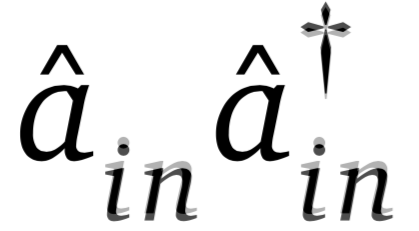
\includegraphics[scale=0.35]{compact}	
	\cprotect\caption{Illustrating the difference between \verb|\mathstrut| and \verb|\phantom{\dagger}|. The light grey letters are the compact version that used \verb|\phantom{\dagger}|.}
\end{figure}


\subsection{square}
To help distinguish between the operator and the indices, the subscript and superscripts can be given in square brackets as well when using the \texttt{square} option.

\DeclareDocumentCommand{\op}{s m O{} O{} O{}}{%
        \IfBooleanTF#1%
        {\linopstylewide{#2}_{\linopsubscript#3}^{\linopspacewide#4^{#5}\linopsuperscript}}
        {\linopstyle{#2}_{\linopsubscript#3}^{#4^{#5}\linopsuperscript}}
}

\DeclareDocumentCommand{\hc}{s m O{} O{} O{}}{%
        \IfBooleanTF#1%
        {\linopstylewide{#2}_{\linopsubscript#3}^{\linopspacewide\linopconjugate#4^{#5}\linopsuperscripthc}}
        {\linopstyle{#2}_{\linopsubscript#3}^{\linopconjugate#4^{#5}\linopsuperscripthc}}
        }

\begin{table}[H]
	\centering
	\begin{tabular}{ll}
		\verb|\op{a}[in][0]| & $\op{a}[in][0]$ \\
		\verb|\hc{b}[out]| & $\hc{b}[out]$ 
	\end{tabular}
\end{table}

\section{Advanced control}
All the options above are set by renewing some custom commands which are

\begin{table}[H]
	\centering
	\begin{tabular}{lll}
		\toprule
		command & default value & description \\
		\midrule
		\verb|\linopstyle| & \verb|\hat| & style of operators\\
		\verb|\linopstylewide| & \verb|\widehat| & style of starred operators\\
		\verb|\linopconjugate| & \verb|\dagger| & symbol used for Hermitian conjugate\\
		\verb|\linopspacewide| & \verb|\>| & spacing in superscript of \verb|op*|\\
		\verb|\linopspacewidehc| & \verb|\:| & spacing in superscript of \verb|hc*|\\
		\verb|\linopsubscript| & \verb|\mathstrut| & equal spacing in subscript \\
		\verb|\linopsuperscript| & \verb|\mathstrut| & equal spacing in superscript of \verb|op|\\ 
		\verb|\linopsuperscripthc| & \verb|\mathstrut| & equal spacing in superscript of \verb|hc|\\
		\bottomrule
	\end{tabular}
\end{table}

These can be changed with \verb|\renewcommand| for even further control.
	
\end{document}
